\documentclass[11pt,letterpaper]{article}
\usepackage[margin=0.90in]{geometry}
\usepackage{amsmath, amssymb}
\usepackage{times}
\usepackage{fancyhdr}
\pagestyle{fancy}
\usepackage{natbib}
\usepackage{titling}
\usepackage{setspace}
\usepackage{bm}
\usepackage{xcolor}
\usepackage{rotating}
\usepackage{graphicx}
%\setlength{\textfloatsep}{-1pt}


\begin{document}
\begin{titlepage}
	\centering
	{\scshape\LARGE McMaster University \par}
	\vspace{1cm}
	{\scshape\Large Final project for Datascience 780\par}
	\vspace{1.5cm}
	{\huge Predicting Diabetes in  Pima Indian Women \par}
	\vspace{2cm}
	{\Large\itshape by Nik Po\v cu\v ca\par}
	\vfill
	Instructor:  \par
	Dr. Sharon McNicholas 

	\vfill

% Bottom of the page
	{\large \today\par}
\end{titlepage}

\doublespacing

\section{Introduction}

Diabetes is an ongoing chronic illness that causes the body to have an inability to process glucose(sugar) by restricting or eliminating the kidney's ability to produce insulin. 
By 2025 the estimated prevalence of diabetes in Canada will increase to 5 million or $12.5 \%$ of Canadians everywhere, not only putting Canadian lives at risk of premature death but cost alone is estimated to increase by $25 \% $ in 2025 \citep{diabetes}. Therefore, the need to accurately predict diabetes is growing with predictive modelling at the forefront. The Pima Indians dataset contains a population of women who were at least 21 years old of Pima Indian heritage and living near Phoenix, Arizona. The population was tested for diabetes according to World Health Organization criteria and data were collected by the US National Institute of Diabetes \citep{pima}. This report contains a thorough set of analyses for the purposes of classifying diabetes based on covariates. First a look at each covariate and description of measurements is provided. Secondly, model methodology and description of model use is discussed. Furthermore, results from both training models and criteria for optimal model selection is provided. Finally, conclusions regarding the feasibility of the utilization of these models are discussed. 

\section{Pima Dataset}

The Pima dataset (Diabetes of Pima Indian Women) taken from the MASS package \citep{pima_d}
in the programming langauge R \citep{Rprog} contains $ 532$ complete records after dropping the (mainly missing) data on serum insulin.  The dataset contains $7$ covariates and $1$ response variable described in Table 1. A variable of particular interest is the pedigree function ($ped$) which provides a numeric feature based on the genetic history of relatives and their relationships to the subject \citep{pima}.


\begin{table}[!h]
\label{covDes}
\caption{Description of covariates in Pima dataset with summary statistics.}
\centering
\begin{minipage}{\textwidth}
\begin{tabular}{|llrrrr|}
\hline
Variable & Description & $\mu$ & $\sigma$ & min & max \\ 
\hline
$npreg$      & number of pregnancies (integer)                                                                                     & 3.52   & 3.31  & 0.00  & 17.00  \\
$glu$   & plasma glucose concentration. (integer)\footnote{count of quantity of plasma after 2 hours} & 121.03 & 30.97 & 56.00 & 199.00 \\
$bp$         & diastolic blood pressure (mm Hg).                                                                                   & 71.51  & 12.30 & 24.00 & 110.00 \\
$skin $      & triceps skin fold thickness (mm).                                                                                   & 29.18  & 10.51 & 7.00  & 99.00  \\
$bmi $       & body mass index (weight in kg/height in m$^2$).                                    & 32.89  & 6.87  & 18.20 & 67.10  \\
$ped$        & diabetes pedigree function \footnote{diabetes mellitus history in relatives and the genetic relationship of those relatives to the patient see \cite{pima} }                                                                               & 0.50   & 0.34  & 0.09  & 2.42   \\
$age$        & age in years. (integer)                                                                                             & 31.61  & 10.75 & 21.00 & 81.00  \\
\hline
$type $      & Yes or No (binary response)                                                & -      & -     & -     & -     \\
\hline
\end{tabular}
\end{minipage}
\end{table}
Furthermore, since each covariate is of a different magnitude, scaling would be beneficial when training a model. 
A concerning observation of a large number of pregnancies totalling to $17$ for a diabetic individual shows a large $bmi$ measurement of $40$. In general, a $bmi$ of 30 or greater is considered to be overweight \citep{diabetes}. Further research into the Pima Indian tribes show a rate of miscarriage among the women which explains the large number of pregnancies for this individual. 
Furthermore, the pairs plot shown in Figure \ref{pairsPlot} displays the skewness of both groups and a heterogeneity within each histogram (see diagonal). In addition, the diabetic group (blue) has a multi-modal shape indicating that there may be more than one sub group within the diabetic group. Correlation coefficients between covariates remain to be relatively low (upper triangle) with $bmi$ and $skin$ having the highest correlation of $0.647$. This is to be expected as body mass index ($bmi$) measures the ratio of weight to height of body, and overweight individuals tend to have a larger tricep skin fold thickness ($skin$). The split between classes is also an issue, Table \ref{count} shows a class imbalance with a 2-1 ratio between normal individuals and diabetic.  
 With independence between covariates established, the dataset is concluded to be of sound quality and relevant to the purpose of classifying diabetes for individuals in a population. 

\begin{figure}
\label{pairsPlot}
\caption{Pairs plot of covariates coloured blue for diabetic and red for normal individuals with correlation coefficients in the upper triangular portion of the pairs plot.}
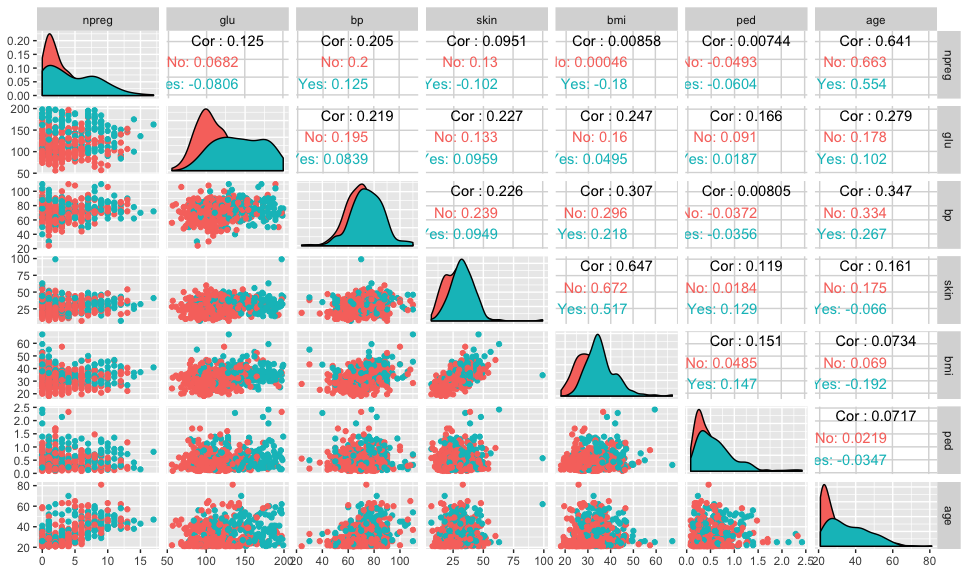
\includegraphics[scale=0.50]{plotgg}
\end{figure}



\begin{table}[!h]
\label{count}
\caption{Counts of individuals for each class.}
\centering
\vspace{10pt}
\begin{tabular}{|r|r|}
\hline
Normal & Diabetic \\ 
\hline
355	&	 177 	\\
\hline
\end{tabular}
\end{table}
\section{Methodology}
As is often in predictive modelling, training is time intensive as the number of possible combinations for model parameters are extremely large. In addition, there are numerous frameworks of evaluation criteria for testing the robustness and accuracy of these models. For the purposes of simplicity an overview in Figure \ref{fig:overview}
demonstrates the methodology used to prepare data, train models, and evaluate model performance. All programming and numerical optimization was done in the R programming environment \citep{Rprog}.

\subsection{Data Preparation}
The Pima dataset was split according to an 80-20 between training set and test set. Of the $80 \%$ in training, it is noted that there are twice as many  normal individuals as diabetic so another bootstrapped training set is created to be trained in parallel with the original sample. Balanced training sets often lead to better model performance on test sets \citep{imbalance}.  Furthermore all covariates are scaled in preparation as each covariate has a different measurement, in doing so, scaling would standardize the impact of each covariate. 

\subsection{Model Methodology}
Three models are considered for the purposes of classification. Due to the skewness of the dataset, mixtures of hyperbolic distributions  from the MixGHD package in R are considered \citep{mixGHD}. For the purposes of prediction, boosted trees are considered to the be the best among other models. Although there have been examples where random forests have an edge, boosted trees are selected for their popularity and effectiveness in data science competitions \citep{gbm}. \subsubsection{Mixtures of Hyperbolic Distributions}

Consider a random vector $\bm{X}$ that emanates from a finite mixture model with $\bm{x} \in \bm{X}$ with $\bm{x}$ as a realization of $ \bm{X}$. Furthermore assume that for the sample space $\Omega$, where $X \in \Omega$ one can partition $\Omega$ into $G$ subgroups $\Omega = \{\Omega_1, \dots ,\Omega_G \}$. Stemming from this the joint distribution of $\bm{X}$ is written as

$$f(\bm{x}| \bm{\theta}) = \sum_{g = 1}^G \pi_g f(\bm{x}| \bm{\theta}_g), $$

where $\pi_g$ denotes the mixing proportion of $g$th group  as a convex combination with $\sum_{g=1}^G \pi_g = 1$. Given an assumption that $\bm{X}$ is of a generalized hyperbolic distribution, then $f(\bm{x}| \bm{\theta}_g)$ is formulated as 

$$ f (\bm{x}| \bm{\theta}_g) = \left[ \frac{ \omega_g + \delta(  \bm{x}, \bm{\mu_g} | \bm{\Sigma}_g  )     }{ \omega_g +  \alpha^{'}_g \bm{\Sigma^{-1}}_g \alpha_g  }\right]^{(\lambda - p/2)/2} \frac{K_{\lambda - p/2} \left( \sqrt{ (\omega_g +  \alpha^{'}_g \bm{\Sigma^{-1}}_g \alpha_g ) (  \omega_g + \delta(  \bm{x}, \bm{\mu_g} | \bm{\Sigma}_g  ))   }    \right)    }{(2 \pi)^{p/2} |\Sigma|^{1/2} K_\lambda(\omega_g) \exp\{ - ( \bm{x} - \bm{\mu}_g)^{'} \bm{\Sigma_g}^{-1} \bm{\alpha}_g\}  } .   $$ Parametrization of $\bm{\theta}_g$ is extremely complicated involving definitions of Bessel functions. For specifics see \cite{hyper}. Furthermore, introducing the concept of a complete data likelihood consider a latent random variable $\bm{Z}_{ig}$ being $1$ when the observation is in group $g$ and $0$ otherwise. The complete-data likelihood of $\bm{\theta}_g$ is written as 

$$L(\bm{\theta} | \bm{x}, \bm{z}) = \prod_{i=1}^n \sum_{g=1}^G \left[  \pi_g f(\bm{x}| \bm{\theta}_g) \right]^{z_{ig}},  $$
where $z_{ig}$ is the realization of $Z_{ig}$. Maximization of parameter vector $\bm{\theta}_g$ is based on the maximum likelihood paradigm. The Expectation Maximization algorithm  is used to find maximum likelihood estimates for the complete data likelihood operating iteratively between E-step and M-steps until a convergence criteria is established \citep{dempster}. In the E-step the a-priori of parameters is used to calculate the a-posteriori as follows 

$$\tau_{ig} = \frac{\hat{\pi}_{ig}  f(\bm{x}| \bm{\theta}_g)  }{ \sum_{k=1}^G \hat{\pi}_{ik}  f(\bm{x}| \bm{\theta}_k) }, $$

where $\tau_{ig} $ is the probability that observation $i$ belongs to group $g$. In the M-step, the complete data likelihood is conditioned on the posteriori where $z_{ig} = \tau_{ig}$. Furthermore, a log transformation is taken arriving at the complete data log-likelihood. Finally derivatives are taken with respect to each component of parameter vector $\bm{\theta}_g$.  The algorithm iterates until convergence is established. For specifics and implementation see \cite{hyper}. Within the complete data likelihood paradigm a semi-supervised learning approach can be taken in the form of Mixture Discriminant Analysis \citep[see][]{mixdist}. 


\subsubsection{Gradient Boosted Trees}
Given a set of data with $n$ observations and $m$ covariates ($\bm{x_i}$) on some set $D = \{ (x_i,y_i) \}$. A tree ensemble uses $K$ additive functions to predict the output of ($y_i$) written as follows 

$$ \hat{y_i}  = \sum_{k=1}^K \lambda f_k(\bm{x}_i), $$ 

where $f_k$ is a regression tree, and $\lambda$ is a shrinkage parameter. Typically when optimizing gradient boosted tree models one devises a Loss function of the following formula 

$$L^{(t)} = \sum_{i=1}^n l(y_i, \hat{y}^{(t-1)}_i + f_k(\bm{x}_i)) + \phi(f_k) $$

Where $\phi(f_k)$ is a penalization term for the complexity of the model \citep[see][for specific implementation]{gradientboost}.

\subsection{Training Methodology}
Training methodology is split between discriminant analysis and gradient boosted trees (gbm). In regards to training a gbm model, the the caret package is one of the best methods  \citep{caret}. The  caret package first selects a measure of model performance (e.g. misclassification rate), and then uses a grid search based method to optimize the hyper parameters (shrinkage, interaction depth, number of trees). To prevent over-fitting $5$ fold cross validation (cv) is considered for the purposes of training more robust models. Within 5 fold cv, the training set is further partitioned in to $5$ equally size sub samples in which a single sub sample is retained as a validation set.  
For performing mixture discriminant analysis, the semi supervised approach is framed through the complete data likelihood as follows 

$$L(\bm{\theta}) =   \prod_{i=1}^k \sum_{g=1}^G \left[  \pi_g f(\bm{x}| \bm{\theta}_g) \right]^{z_{ig}} \times \prod_{j=k+1}^n \sum_{h=1}^H \left[\pi_h\phi(\bm{x}_j| \bm{\theta}_h) \right].$$

Here, all of the observations of $\bm{x}$ are used to predict labels for the missing $\bm{x}_{k+1}, \hdots ,\bm{x}_n$ \citep{mixdist}. Class prediction is based on the EM algorithm with a hard classification as follows:

$$z_{jh} = \arg \max_{h \in H} \tau_{ih}  , \quad \tau_{ih} = \frac{\hat{\pi}_{ih}  f(\bm{x}| \bm{\theta}_h)  }{ \sum_{h=1}^H \hat{\pi}_{ih}  f(\bm{x}| \bm{\theta}_h) }. $$


                       

\subsection{Evaluation Methodology}
Evaluating model performance is again split between selection of mixture models and gbm models. For the choice of the best mixture model the Bayesian index criterion (BIC) is considered. The formula for BIC is 

$$\textbf{BIC} = \log(n) k - 2 \log(\hat{L}), $$

where $n$ is the number of observations, $k$ is the number of parameters and  $\hat{L}$ is the maximized likelihood after convergence of EM was achieved.  Mixture models are ran for groups 1:$G$, and the model with the lowest BIC is selected to be the best.  
Evaluation of gbm models is based on the adjusted rand index criterion (ARI). ARI is calculated using the following formula :


$$ARI = \frac{ \sum_{ij} \binom{n_{ij}}{2} - [\sum_i \binom{a_i}{2} \sum_j \binom{b_j}{2}] / \binom{n}{2} }{ \frac{1}{2} [\sum_i \binom{a_i}{2} + \sum_j \binom{b_j}{2}] - [\sum_i \binom{a_i}{2} \sum_j \binom{b_j}{2}] / \binom{n}{2} }, $$

where $a_i$ is the ith row sum, and $b_j$ is the jth column sum \cite{mixdist}.  In summary, ARI can be thought of as the ``corrected for chance" of the number of object pairs that are either in the same group or in different groups, across all partitions divided by the total number of object pairs.

\section{Results}

The result section is split into two parts. First, training results comparing model performance across all variations of models and datasets are discussed. Secondly, the optimal model is chosen and further analysed in the context of classifying diabetes. 

\subsection{Training Results}

Over six variations of both model and dataset were done, the results of each model performance is listed in Table \ref{modelPerf}. Training parameters for gbm models is set to a 5 fold cross validation, a grid of $1-500$ for number of trees, and two settings of shrinkage parameters of $0.01$ and $0.001$. In regards for training mixture models, initializations for the EM algorithm uses kmeans to initialize memberships \citep{mixGHD}.  Furthermore, for the feature generation using hyperbolic models, only $G=\{1,\hdots,6\}$ were considered. Boosted tree models had the best results with the following tuneing parameters: n.trees = 311, interaction.depth = 2, shrinkage = 0.01 and n.minobsinnode = 10.   However, given a boosted tree model with a feature map the best ARI measure is with parameters n.trees = 376, and interaction.depth = 2. Table \ref{modelPerf} shows that  bootstrapping  only improved results for discriminant analysis using hyperbolic models. Bootstrapping did not affect any ARI or gradient boosted tree models. Finally, the best model with an ARI of 0.3546  is using Boosted trees with a hyperbolic feature map. Within this framework, a mixture of hyperbolic distributions are used to develop a vector of assigned classes. The number of classes does not necessarily have to be the same number of types needed for prediction. The hyperbolic feature generated five groups in which were now considered as covariates in the boosted tree. 


\begin{table}[!h]
\centering
\caption{Model performance results with ARI and class error over all six variations. }
\vspace{5pt}
\label{modelPerf}
\begin{tabular}{|l|rr|}
\hline\hline
Method                                         & ARI    & Class Error \\
\hline
DA Hyperbolic                                  & 0.1974 & 0.2710      \\
DA Hyperbolic + Boostrap                       & 0.2203 & 0.2617      \\
Boosted Trees                                  & 0.3532 & 0.1963      \\
Boosted Trees + Boostrap                       & 0.3532 & 0.1963      \\
Boosted Trees + Hyperbolic Feature             & $\bm{0.3546}$ & $\bm{0.1963}  $   \\
Boosted Trees + Hyperbolic Feature + Bootstrap & 0.3546 & 0.1963     \\
\hline\hline
\end{tabular}
\end{table}


\subsection{Boosted Tree with Hyperbolic Feature Results}

The best model is a gradient boosted tree with an extra covariate that was generated from a hyperbolic mixture distribution. First, a mixture of hyperbolic distributions is fit in which five groups were found .The mixture model has a BIC of  $7665$ and Table \ref{classTable} as its classification table. Classes 1, 2, and 5, have a very skewed spit between types of individuals. This is a good indication that the covariate could potentially predict whether the individual is diabetic or not. Secondly, the vector of memberships arising from this mixture model is selected to be an extra covariate in fitting a gradient boosted tree model with parameters:  n.trees$=371$ ,
                 interaction.depth=$1$, and
                 shrinkage = $0.01$. The classification table (Table \ref{classTable}) shows the gradient boosted tree results with a total of 20 misclassified individuals.  The ARI measurement of the test set is $0.3775$ which is slightly better than the training ARI of $0.3546$. Furthermore, the relative influence of each covariate shows interesting results (Table \ref{relInflu}). The $glu$ covariate, which is the count of glucose plasma in the blood accounts for over $51 \%$ of the predictive power in the model with $age$ following shortly after with only $18\%$. Lastly the $hyper$ covariate that was generated from modelling hyperbolic mixtures in an unsupervised fashion accounted for less then half a percent of the predictive influence. The ROC curve shown in Figure \ref{rocr} displays predictive results between false positive rate and true positive rate. The curve shows very poor prediction, the false positive rate is very high in comparison to the true positive rate. Meaning that the model is more likely to classify someone with diabetes rather than without. The mirrored plot featuring the true negative rate and false negative rate shows similar results when comparing the model's predictive performance. No matter which way you look at it, the model's performance is unsatisfactory due to the incidents of misclassification. 

\begin{figure}
\label{rocr}
\caption{ROC curve (left)  for Boosted Tree Model with Hyperbolic Features as well as a true negative vs false negative rate plot (right).}
\centering
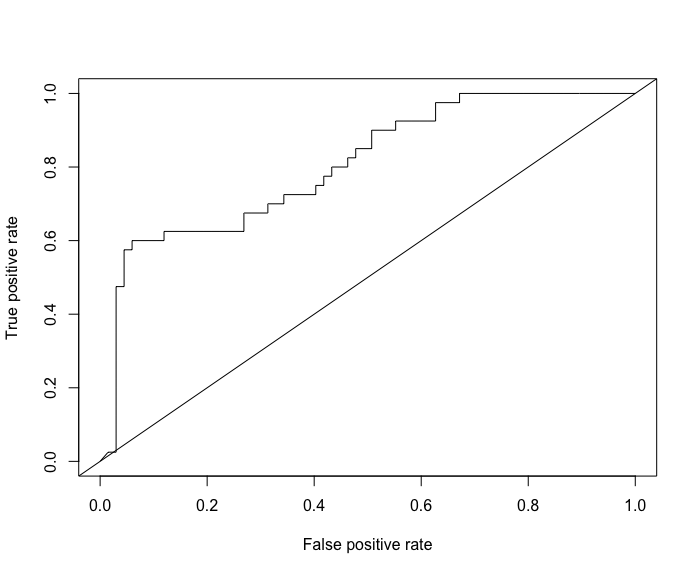
\includegraphics[scale=0.3]{rocr}
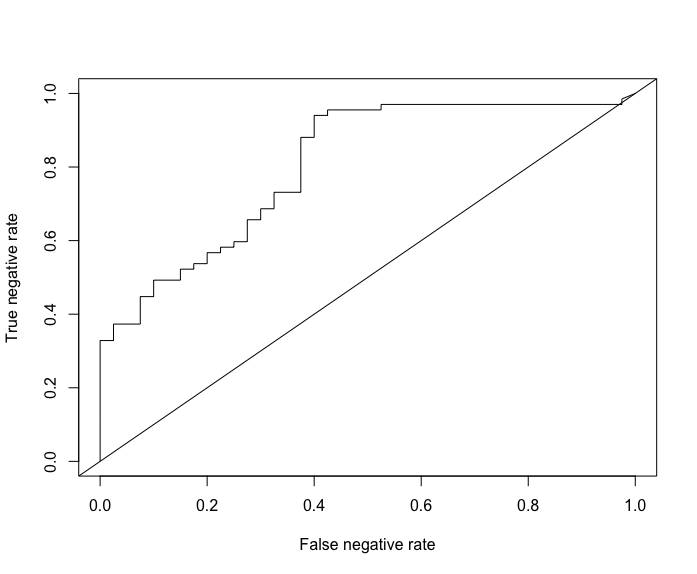
\includegraphics[scale=0.3]{trueNeg}
\end{figure}

\begin{table}
\label{classTable}
\caption{Classification table for mixture of hyperbolic distributions (left) and gradient boosted trees (right), vertical (0,1) is positive for diabetes and horizontal is mixture class label.}
\vspace{8pt}
\centering
\begin{tabular}{|r|rrrrr|}
\hline\hline
Classes & 1  & 2  & 3  & 4  & 5  \\
\hline
0       & 8  & 93 & 76 & 34 & 77 \\
1       & 17 & 20 & 54 & 31 & 15 \\ 
\hline \hline
\end{tabular}
$\quad\quad$
\begin{tabular}{|r|rr|}
\hline\hline
          & \underline{Predicted} &   \\
\underline{True Values} & 0         & 1  \\
\hline
0           & 64        & 3  \\
1           & 17        & 23 \\
\hline\hline
\end{tabular}
\end{table}

\begin{table}[!h]
\centering
\label{relInflu}
\caption{Relative influence of each covariate on boosted tree prediction in percetages. }
\vspace{5pt}
\begin{tabular}{|l|llllllll|}
\hline\hline 
Variable                & glu    & age    & bmi    & ped   & npreg & skin  & hyper & bp    \\ 
\hline
Relative Influence (\%) & 51.480 & 18.203 & 13.484 & 9.989 & 5.107 & 1.253 & 0.484 & 0.000  \\
\hline\hline
\end{tabular}
\end{table}





\section{Conclusions}
Overall, providing an extra feature for a boosted tree only slightly improved performance of ARI. The class error on the test set of  $18.69 \%$ meaning that over $20$ individuals were misclassified by the model out of $107$. In conclusion, although the mixture models are robust and can account for skewness in the data, boosted trees supersede them in predictive power. Furthermore, an improvement in predictive power could be made with using labels derived from an unsupervised model. With respect to predicting diabetes in the Pima Indian women, reliably predicting diabetes in individuals using the covariates listed above is unsatisfactory. There are too many false negatives predicted from the model meaning that many individuals who do indeed have diabetes would not be detected reliably from the model. In addition, the feasibility of collecting blood samples and pedigree information is called into question as expenses from lab tests are often costly. Future work should look into finding less invasive procedures to determine diabetic status.  



\begin{sidewaysfigure}
\section{Appendix}
\label{fig:overview}
\caption{Methodological Overview}
\centering
\vspace{20pt}
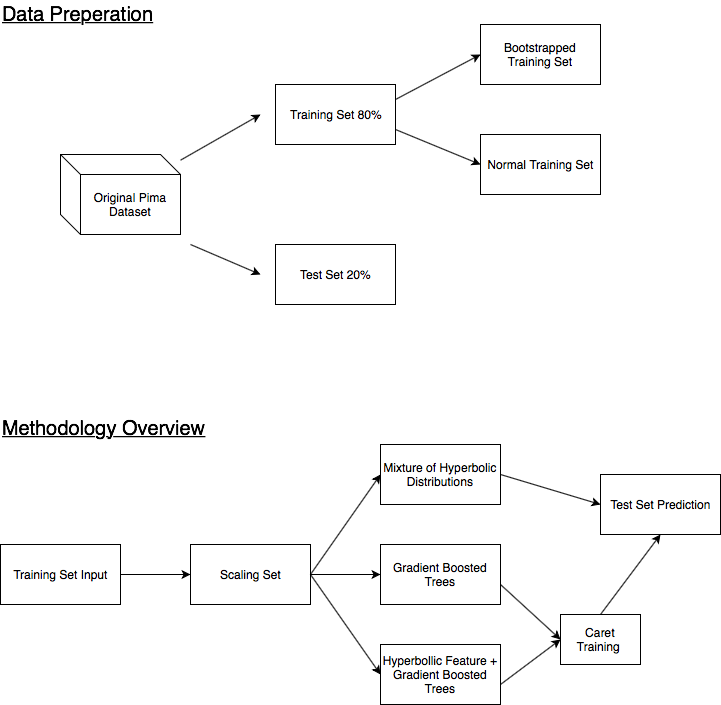
\includegraphics[scale=0.45]{MethodOverview}
\end{sidewaysfigure}


\newpage
\bibliographystyle{elsart-harv}
\bibliography{final_b}
 
\end{document}


